% !TEX program = xelatex
\documentclass[11pt,a4paper]{ctexart}
\usepackage[margin=2.4cm]{geometry}
\usepackage{graphicx}
\usepackage{booktabs}
\usepackage{float}
\usepackage{hyperref}
\usepackage{amsmath}
\usepackage{fontspec}
\setmainfont{Times New Roman}
\setCJKmainfont{Microsoft YaHei}
\setCJKsansfont{Microsoft YaHei}
\usepackage{caption}
\captionsetup{font=small,labelfont=bf}
\hypersetup{colorlinks=true,linkcolor=blue!50!black,urlcolor=blue!50!black}

\title{\textbf{基于 MarsWorkbench 的 SHERLOC 数据处理流程}\\ \large ——从 PDS 原始档案到逐点矿物判读}
\author{MarsWorkbench 项目组}
\date{2026 年 11 月}

\begin{document}
\maketitle

\begin{abstract}
SHERLOC 是毅力号火星车机械臂上的深紫外拉曼与荧光光谱仪。本文介绍本地离线工作台
MarsWorkbench 对其 PDS 公开数据的完整处理与判读流程：预处理管线中每一步的物理作用与
跳过判据、候选矿物判读与验证方法、以及软件工作台的实现。全部流程在本地离线运行、可复现，
并以已发表文献的逐靶对账作为检验基准。文中所有插图均由本软件对真实 PDS 数据处理后生成。
\end{abstract}

\tableofcontents

\section{引言：SHERLOC 仪器与科学目标}

\subsection{仪器概况}
SHERLOC（Scanning Habitable Environments with Raman \& Luminescence for Organics and
Chemicals）安装在毅力号火星车机械臂 turret 上，使用 248.6\,nm 深紫外激光对目标进行
拉曼与荧光联合观测，用于识别有机物与矿物信号。配套的 ACI（自动对焦显微成像仪）提供
逐点级灰度显微影像，WATSON 提供彩色工程影像 [待补：仪器论文引文]。

\subsection{观测方式}
SHERLOC 以逐点扫描方式观测：一次扫描覆盖目标上规则排列的点阵（精细扫描典型为
100 点，普查扫描可达 1296 点）。每个点采集一条深紫外光谱，分为拉曼区（Region 1）
与两个荧光区（Region 2/3）。

\subsection{PDS 数据产品}
行星数据系统（PDS）公开发布 SHERLOC 的原始与处理产品，包括原始谱表、坐标表、
图像清单以及处理后的光谱产品，配套 XML 标签。本文数据取自 PDS 公开档案
（随包示例与本地练习数据树）。

\subsection{本文范围声明}
本文描述的判读结果均为\textbf{检出候选}，不构成矿物鉴定；在缺少独立盲标真值的情况下，
本工具不宣称矿物鉴定准确率、假阳性率或假阴性率。

\section{数据与预处理方法}

\subsection{预处理管线总览}
MarsWorkbench 的 SHERLOC 预处理管线由七个可选步骤组成，每一步都可以独立开关；
当某步骤对当前数据不适用时，管线会\textbf{自动跳过并在日志中给出理由}，
而不是静默执行。图~\ref{fig:ui} 为工作台界面，右侧日志区逐条给出各步骤的执行情况。

\begin{figure}[H]
  \centering
  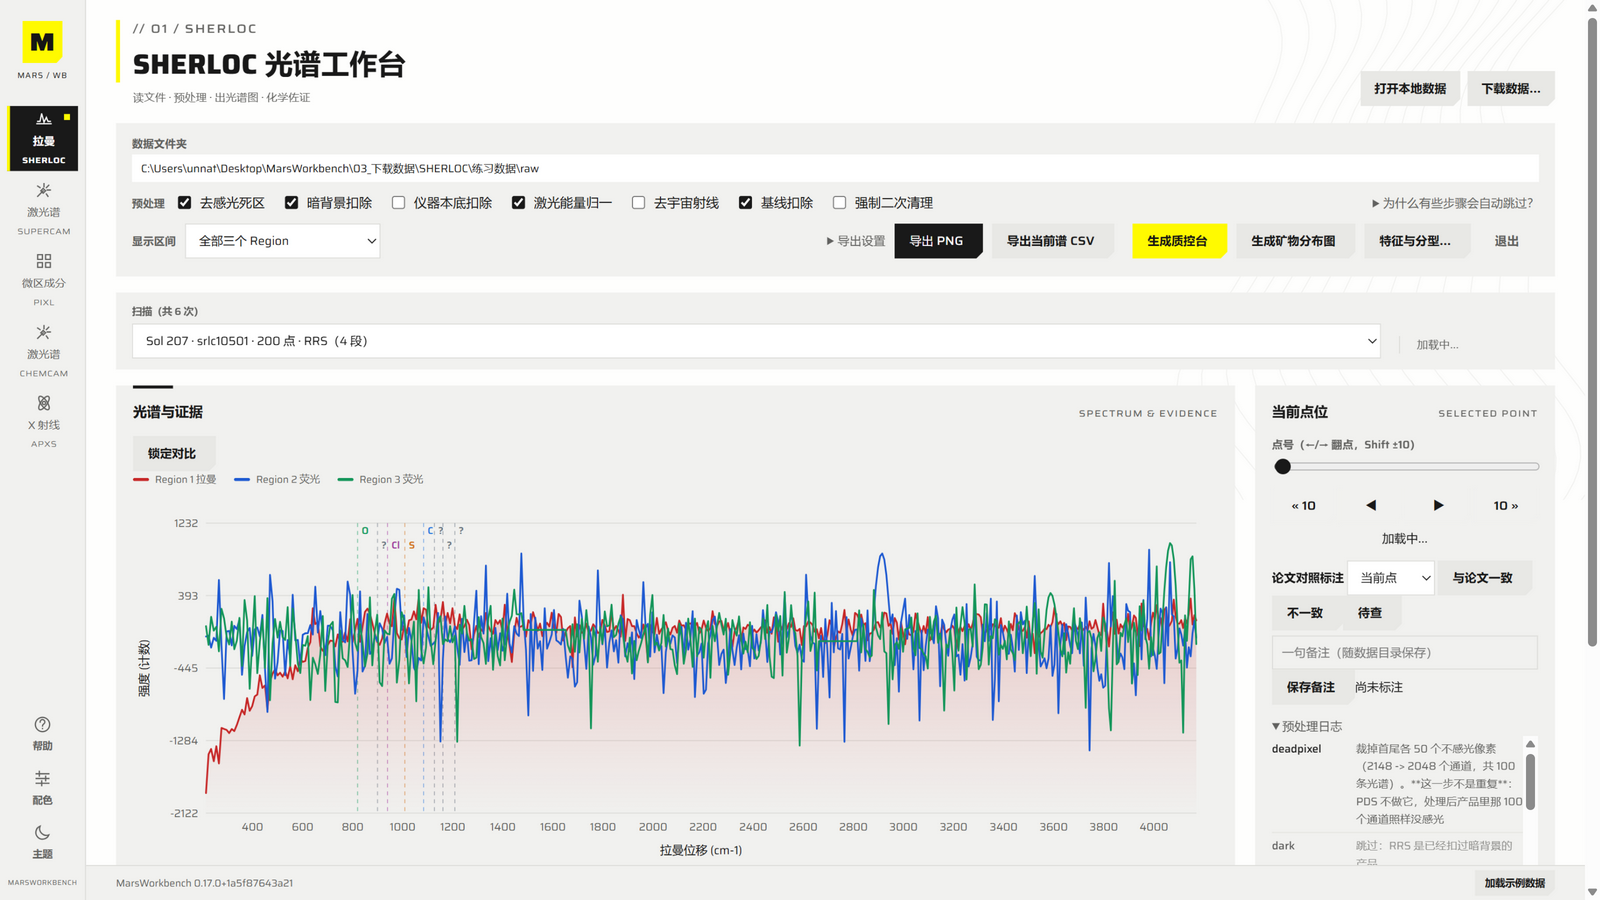
\includegraphics[width=\textwidth]{figs/fig_ui_workbench.png}
  \caption{SHERLOC 光谱工作台。左侧为仪器导航，中部为光谱与证据区（三 Region 叠加），
  右侧为当前点位与论文对照标注，底部日志逐条说明各预处理步骤的执行或跳过理由。}
  \label{fig:ui}
\end{figure}

\subsection{去感光死区}
SHERLOC 光谱首尾各有 50 个不感光像素，物理上不产生有效信号。此步骤将其裁除
（2148$\to$2048 通道）。PDS 原件不做此处理——处理后产品中这 100 个通道依旧
没有感光，因此该步骤并非重复劳动。

\subsection{暗背景扣除}
若数据配对有暗背景帧（ERA$-$ERB），则逐 Region 相减。本文使用的 RRS 类产品
已在星上扣除暗背景，管线检测到这一点后自动跳过并说明，避免二次扣除引入偏差。

\subsection{激光能量归一}
逐发激光能量波动会导致谱强度不可比。label 中标注 LASER-NORMALIZED 的产品
已在星上归一化，管线再次检测到后跳过——再归一次等于把数据改两遍。

\subsection{去宇宙射线（跨发 MAD）}
高能粒子会在单发谱上留下孤立尖峰。管线以跨发中位数绝对偏差（MAD）逐通道判定，
将尖峰替换为跨发统计值，保留其余信息。该步骤逐发独立进行；未开启时，
原始谱中的尖峰按原样保留（不作假装干净的处理）。

\subsection{仪器本底扣除}
SHERLOC 的无镀膜 SiO$_2$ 光学件在 490/800/1055/1190\,cm$^{-1}$ 处产生固定本底
拉曼，单谱信噪比低于 1 而不可见，但在逐点统计时显现，并与橄榄石识别峰
（815--865\,cm$^{-1}$）直接重叠 [待补：Jakubek 2024 引文]。

本工作台实现收纳臂暗天空法：以火星车未展开时的暗天空扫描构造仪器本底谱，
按缩放因子 $M$ 相减。$M$ 只在 800\,cm$^{-1}$ 主带窗内用中位数比值估计，
本底谱覆盖范围内全波段按形状缩放相减（官方做法），覆盖外通道保持原值。
实测 Sol 293 数据 $M=1.409$，覆盖 100\%，扣除后主带中位数趋近于零。
图~\ref{fig:instbkg} 给出扣除前后的对比。该步骤定位为\textbf{判读对照工具}，
不是定量步骤。

\begin{figure}[H]
  \centering
  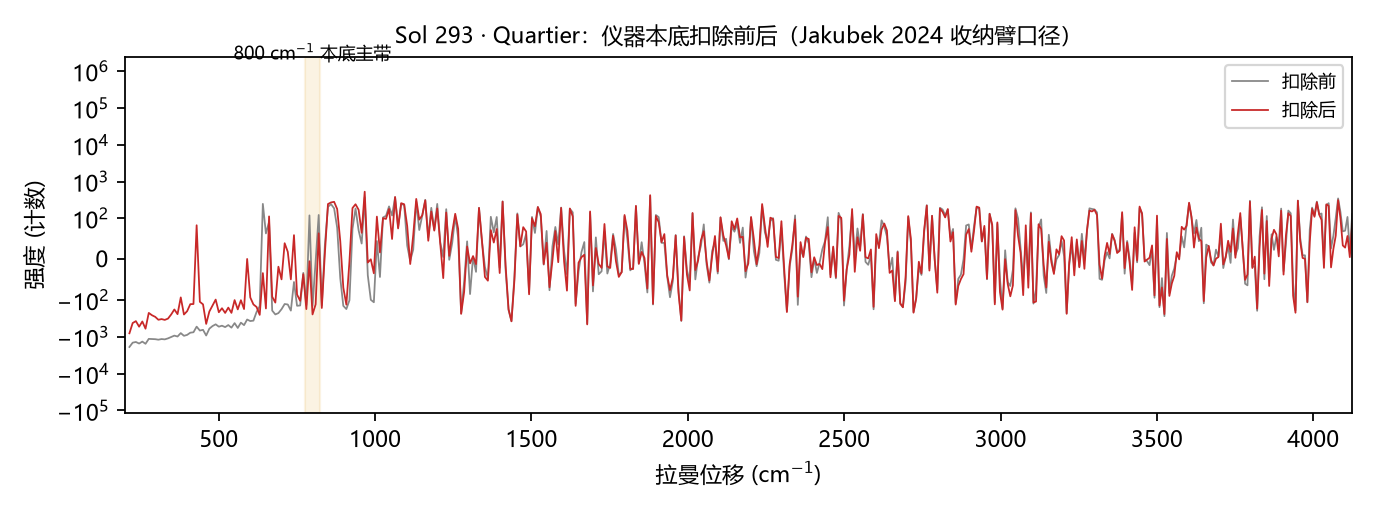
\includegraphics[width=\textwidth]{figs/fig_instbkg.png}
  \caption{仪器本底扣除前后对比（Sol 293，Quartier）。橙色阴影为 800\,cm$^{-1}$
  本底主带位置。}
  \label{fig:instbkg}
\end{figure}

\subsection{基线扣除}
拉曼光谱中的荧光背景以宽包络形式存在，不扣除则几个波数宽的拉曼带完全不可见。
管线在 800--4000\,cm$^{-1}$ 区间以迭代多项式（5 次）拟合基线并扣除。
PDS 原始产品从不扣基线，因此该步骤同样不是重复劳动。

\subsection{强制二次清理（可选）}
对信噪比极差的扫描，可叠加一轮更激进的去尖峰与平滑；默认关闭。

\subsection{管线契约小结}
预处理遵循三条原则：\textbf{已处理不重做}（检测产品标注后自动跳过）、
\textbf{缺输入不硬算}（如无暗帧则明确跳过）、\textbf{每步留痕}（日志逐条给出
执行/跳过理由）。这使「所见即所得」——预览与导出共用同一套处理链。

\section{判读与分析方法}

\subsection{候选矿物峰组与逐点分类}
管线将观测的点阵组织为聚类，每个聚类给出观测峰位与点数，再对照已知矿物拉曼
峰位表给出\textbf{候选}类别（如橄榄石 $\sim$830\,cm$^{-1}$、碳酸盐
$\sim$1085\,cm$^{-1}$）。图~\ref{fig:candidates} 为 Sol 207 平均谱上的
候选检出示意。

\begin{figure}[H]
  \centering
  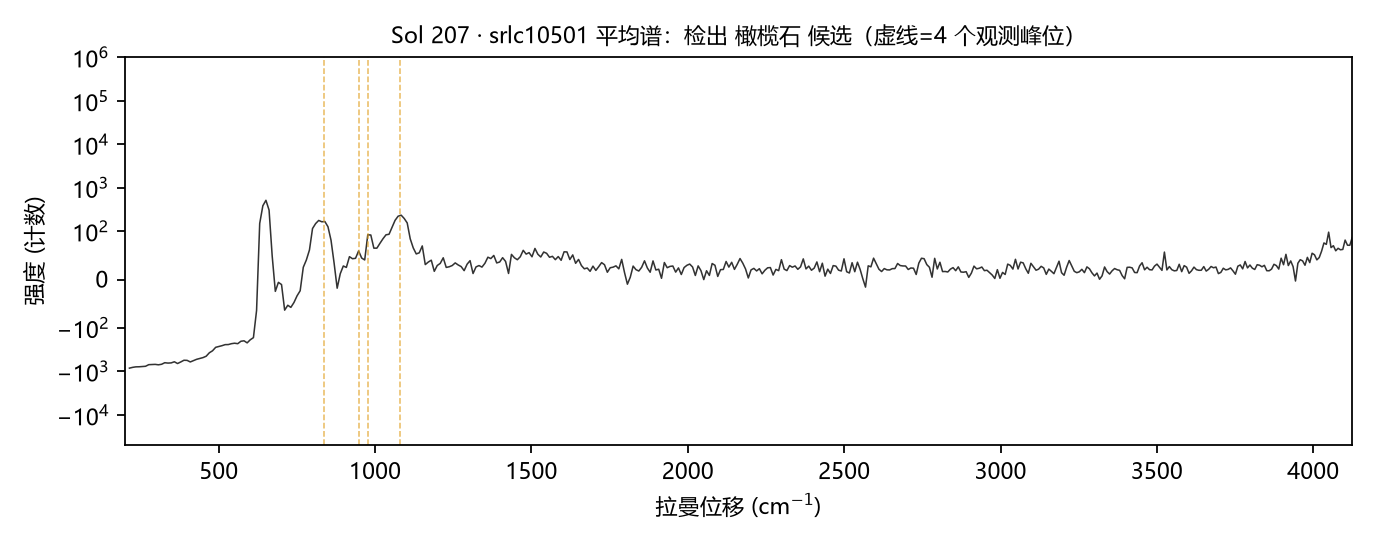
\includegraphics[width=\textwidth]{figs/fig_candidates.png}
  \caption{Sol 207 srlc10501 平均谱与候选矿物峰位（虚线）。}
  \label{fig:candidates}
\end{figure}

\subsection{扫描级兜底}
单点信噪比不足时，管线对整次扫描做聚合分析给出扫描级候选——防止「单点看不见
但扫描整体看得见」的信号被漏掉；同时对已知零信号对照扫描设置上限断言。

\subsection{特征与分型}
工作台提供 A/B 双窗口积分面积比（如碳酸盐的 1060--1110 与 990--1030\,cm$^{-1}$）、
信噪比门槛与聚类分型，输出空间分布图与 HTML 分型报告。需要强调：积分面积不是
矿物含量，类型编号不是矿物鉴定。

\subsection{跨仪器对照}
毅力号上 SuperCam 的 LIBS 点若与 SHERLOC 扫描同址，工作台会并排显示元素证据；
好奇号 APXS 的官方氧化物表也可作比值级对照。跨仪器同址比较不证明共靶。

\subsection{空间分布图}
以 ACI 灰度影像为底图，将逐点矿物归属叠加显示。缺图时保留成分表与报告，
不生成虚构底图。

\section{验证与对账}

\subsection{合成谱护栏}
预处理与判读逻辑由合成数据护栏覆盖（18 项断言）：本底缩放因子 $M$ 的恢复精度、
减除后真实峰位保持、部分覆盖时覆盖外通道逐位不变、缺文件/坏 JSON 的安全降级等。

\subsection{文献逐靶对账}
将软件分类输出与已发表结论逐靶对照（Sun 2023；Corpolongo et al.\ 2023）：
可判类目 14 个，复现 7 个——其中 3 类（长石/绿泥石/层状硅酸盐）经软件粗类
silicate 映射命中，软件实际区分的细类为碳酸盐、橄榄石、硅酸盐。
对照靶点包括 Garde（sol 207）与 Alfalfa（sol 370）等 [待补：引文页码]。

\subsection{已知缺口与假阳性留档}
论文报过而软件报不出的类别（如高氯酸盐或磷酸盐的细分）按已知缺口留档，
只提示不判失败；历史上对照扫描出现的假阳性也有单独记录——这些「做不到」
与「做得到」同样透明。

\subsection{数据版本演进的发现}
PDS 16.0 版（2026-08-11）对处理产品做了重处理。重下载后，对照扫描
（sol 141/181）出现了零星量级的候选检出（$\le$9 点）——这是数据版本演进
所致，按已知差异注记降级处理，不判失败也不隐藏。

\section{软件实现：MarsWorkbench 的 SHERLOC 工作台}

\subsection{架构}
工作台为纯 Python 本地应用（numpy/pandas 必需，astropy/opencv 为可选库），
通过本地 HTTP 服务驱动浏览器界面，\textbf{完全离线}。依赖分层：标准版缺
可选库时仅警告、对应功能显式跳过，不崩溃。

\subsection{功能}
\begin{itemize}
  \item 数据加载：PDS 原名与配对 XML 标签，按目标/sol/序列号组织观测
  \item 逐点导航与三 Region 叠加显示，缩放与锁定对比
  \item 预处理开关（每步带理由日志）与论文对照标注（随数据保存）
  \item 导出：处理谱 CSV、当前点/全观测 PNG、逐点质控报告
  \item 特征与分型面板（A/B 面积比、SNR 门槛、聚类分型、空间图）
  \item 矿物分布图（ACI 底图叠加，无底图模式如实标注）
\end{itemize}

\subsection{质控台}
一键生成全部观测的逐点质控报告（HTML），汇总每个扫描的检出候选与判据说明。
图~\ref{fig:qc} 为 Sol 207/370 六次观测的质控台汇总：绿色为有检出候选的观测，
红色为确认无信号的观测（如 1 点定标小扫描），判据（峰宽须达仪器分辨率下限、
SNR$>3$）直接写在页面上。

\begin{figure}[H]
  \centering
  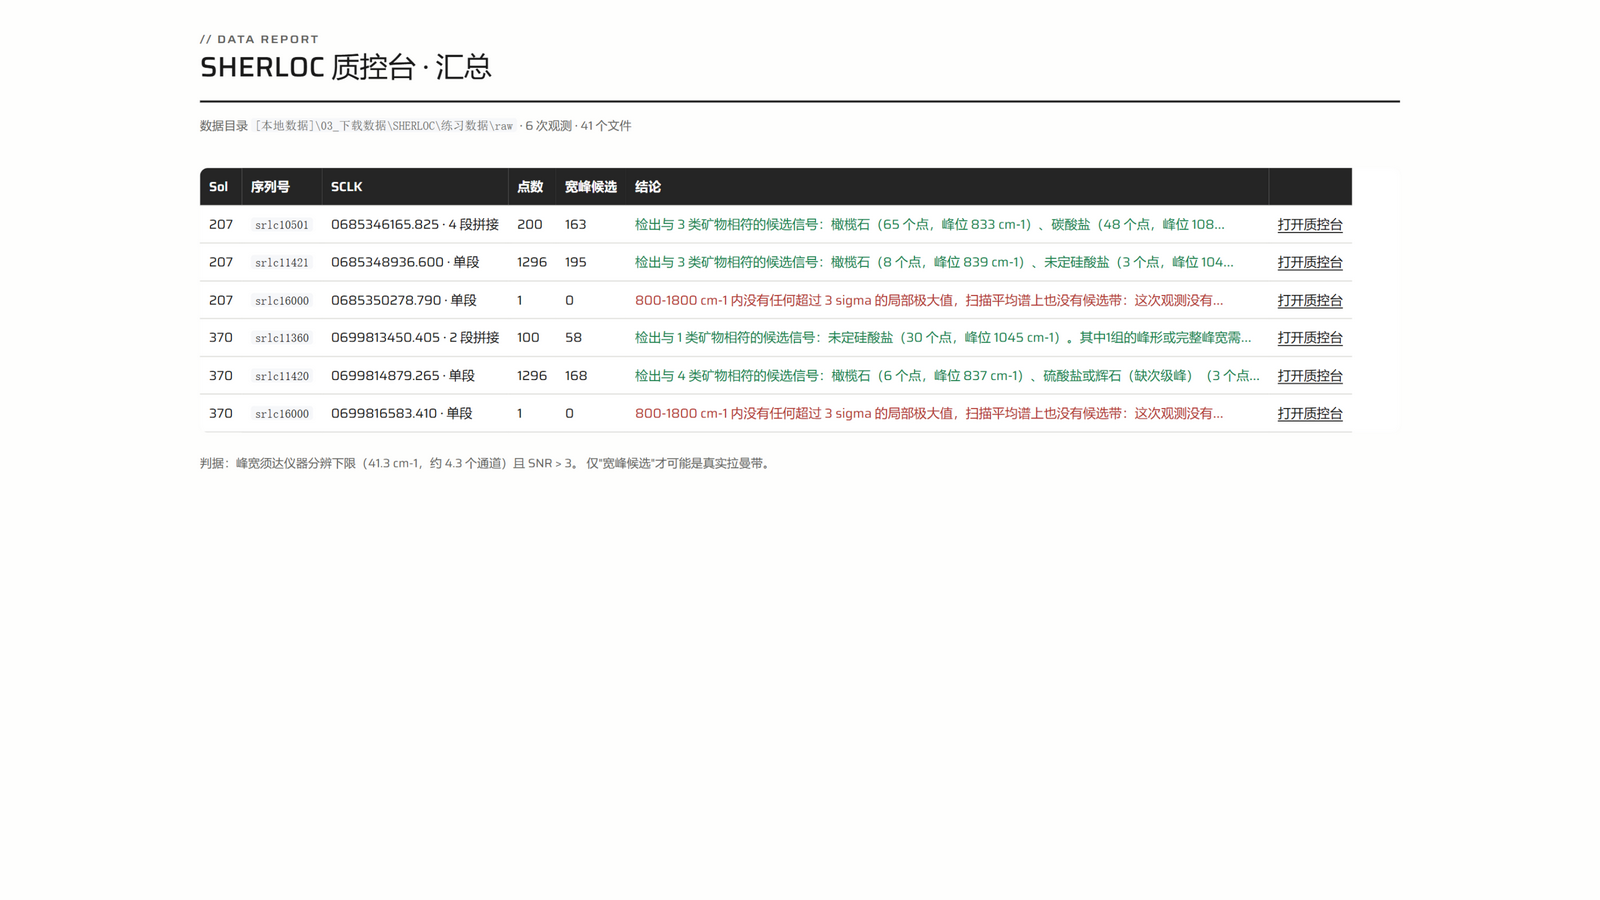
\includegraphics[width=\textwidth]{figs/fig_qc_index.png}
  \caption{质控台汇总页：6 次观测的逐扫描结论与判据。}
  \label{fig:qc}
\end{figure}

\subsection{可复现性}
所有冻结数值基准随代码分发，任何人可重跑三套检查（发行护栏 19 条 436 项、
数据审计 26 项、文献定量对账 24 项）验证本文数字。

\section{案例演示}

\subsection{Sol 207 Garde：200 点扫描全流程}
以 Garde 靶点（Séítah 组）的 200 点扫描为例：预处理日志显示死区裁剪执行、
暗背景与激光归一按产品标注跳过、基线扣除执行；平均谱上检出碳酸盐
（48 点，峰位 $\sim$1085\,cm$^{-1}$）与橄榄石（65 点，峰位 $\sim$833\,cm$^{-1}$）
候选，与已发表结论一致。图~\ref{fig:regions} 为该点三 Region 叠加谱。

\begin{figure}[H]
  \centering
  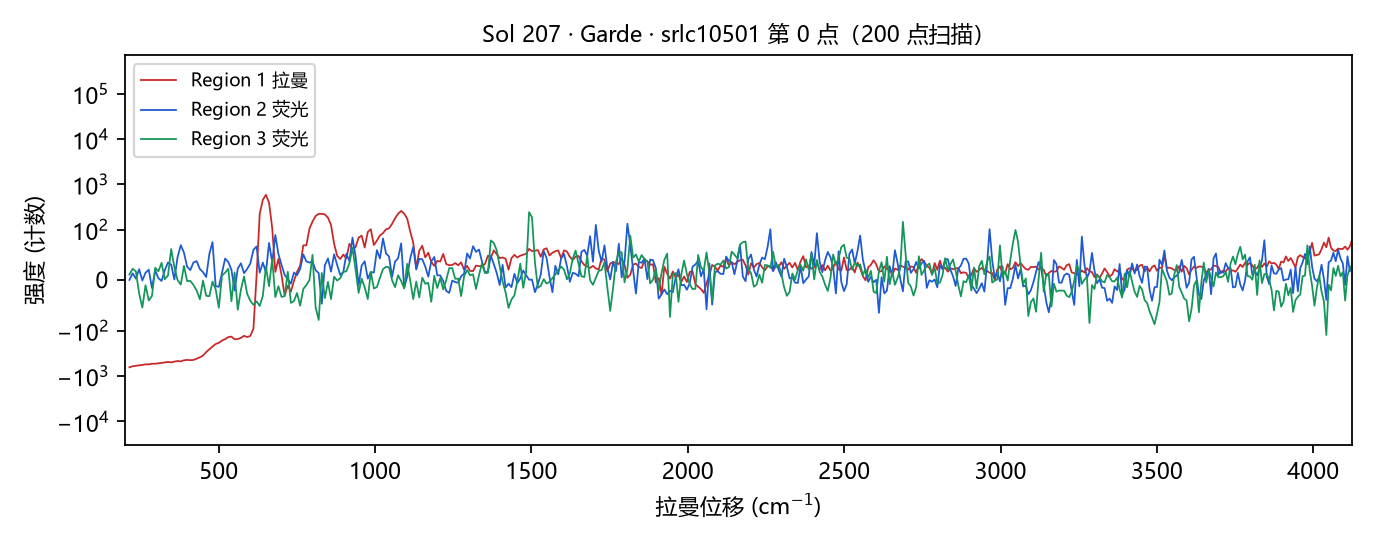
\includegraphics[width=\textwidth]{figs/fig_regions.png}
  \caption{Sol 207 srlc10501 第 0 点的三 Region 叠加谱（基线扣除后）。}
  \label{fig:regions}
\end{figure}

\subsection{预处理各步的作用：单点对比}
图~\ref{fig:steps} 以同一单点展示预处理各步的效果：原始谱中荧光背景包络
完全掩盖拉曼带；基线扣除后 800--1200\,cm$^{-1}$ 观察窗内的结构显现。

\begin{figure}[H]
  \centering
  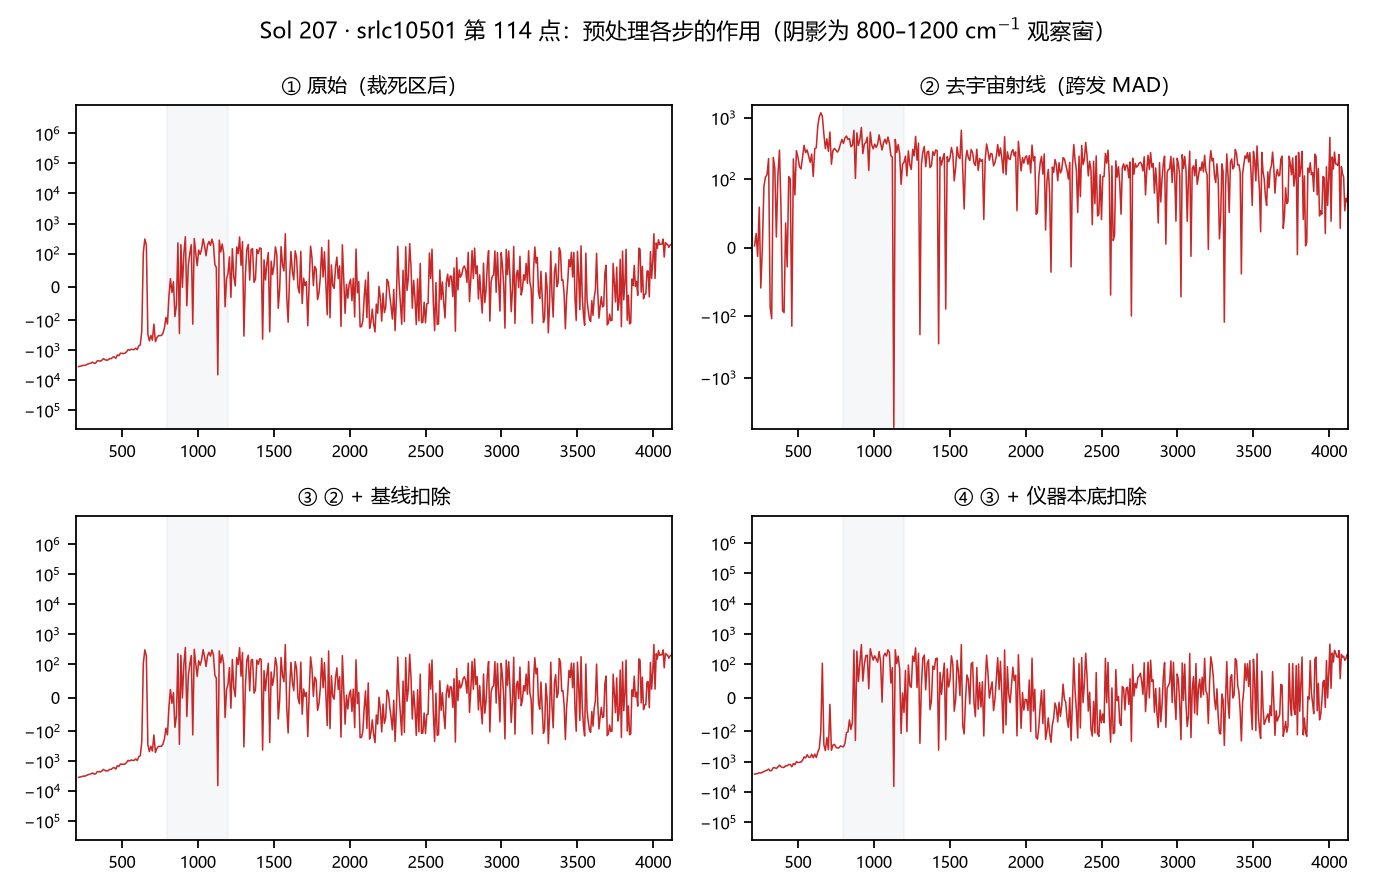
\includegraphics[width=\textwidth]{figs/fig_preproc_steps.png}
  \caption{预处理各步的作用（Sol 207 srlc10501，单点）。}
  \label{fig:steps}
\end{figure}

\subsection{Sol 370 Alfalfa：G 带与扫描分组}
Alfalfa 靶点的 G 带有机质通道（$\sim$1604\,cm$^{-1}$）实测信噪比 12.6$\sigma$；
扫描分组结构断言（多段拼接、对照扫描）全部通过。

\subsection{空间分布图}
图~\ref{fig:distmaps} 为工作台生成的矿物分布图样例（无底图模式）。

\begin{figure}[H]
  \centering
  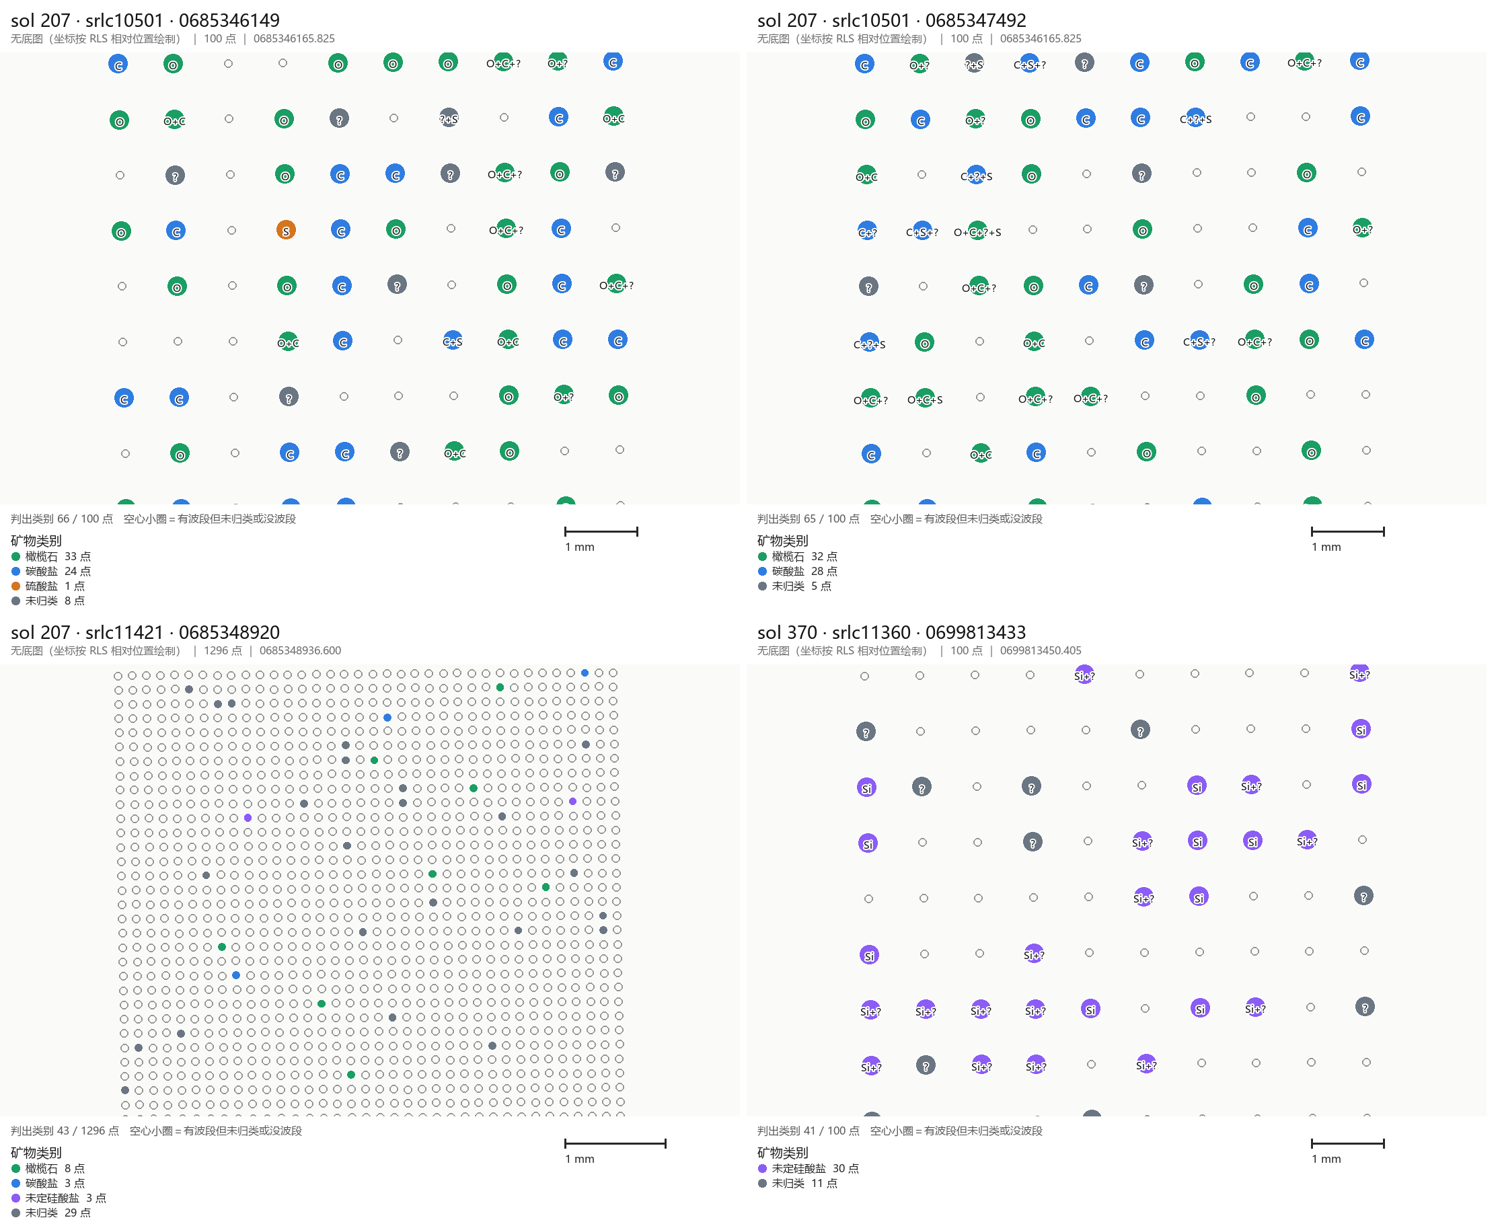
\includegraphics[width=0.85\textwidth]{figs/fig_distmaps.png}
  \caption{矿物分布图样例（4 次观测，无底图模式如实标注）。}
  \label{fig:distmaps}
\end{figure}

\section{结论与展望}

本文展示了基于 MarsWorkbench 的 SHERLOC 数据完整处理链：从 PDS 原始档案出发，
经逐步预处理（每步有明确作用与跳过判据）、候选矿物判读与验证，到工作台交互
与导出，全程本地离线、可复现。局限：判读结果为候选性质，尚无独立盲标真值；
部分论文靶点的原始数据未随本仓库分发。展望：引入 PIQUANT 类定量交叉验证、
扩充论文靶点至全部已发表研磨斑。

\appendix

\section{预处理跳过判据速查表}

\begin{table}[H]
\centering\small
\begin{tabular}{llp{7cm}}
\toprule
步骤 & 跳过条件 & 说明 \\
\midrule
去死区 & 恒执行 & 首尾各 50 个不感光像素 \\
暗背景 & 无配对暗帧 / RRS 类 & RRS 已扣暗背景 \\
激光归一 & label 标注已归一 & 再归一次等于改两遍 \\
去宇宙射线 & 未开启 & 原始尖峰原样保留 \\
仪器本底 & 未开启 / 无本底谱 / 波长不齐 & 收纳臂暗天空法 \\
基线 & 有效波段太窄 & 800--4000 cm$^{-1}$ \\
\bottomrule
\end{tabular}
\caption{预处理步骤与跳过判据}
\end{table}

\section{数据与文献来源}

数据来自 NASA PDS 公开档案（mars2020\_sherloc bundle）。方法与对照文献：
Corpolongo et al.\ 2023（SHERLOC 首年结果）、Jakubek et al.\ 2024（仪器本底）、
Sun et al.\ 2023（毅力号首年概览）、以及 PDS SIS 文档 [待补：完整引文与 DOI]。
NASA 标识不代表对本工具的认可。

\end{document}
